\documentclass[12pt]{article}

\usepackage[utf8]{inputenc}
\usepackage[T1]{fontenc}
\usepackage{graphicx}
\usepackage{xcolor}
\usepackage{tabu}
\usepackage[table]{xcolor}
\usepackage{float}

\usepackage{tikz}
\usepackage{calc}
\usepackage{booktabs}


% colors
\definecolor{color1}{HTML}{000060}
%\definecolor{color1}{HTML}{8C260F}
\definecolor{color2}{HTML}{333333}


% fonts
\usepackage{fontspec}
\defaultfontfeatures{Mapping=tex-text}
\setmainfont
[BoldFont=Lato-Bold.ttf,
ItalicFont=Lato-Italic.ttf,
BoldItalicFont=Lato-BoldItalic.ttf]
{Lato-Regular.ttf}
\newfontfamily\headingfont[ItalicFont=Lato-BlackItalic.ttf]{Lato-Black.ttf}
%%%

\usepackage{geometry}
\geometry{a4paper,
hmargin=20mm,vmargin=20mm,
head=0ex,foot=3ex}

\linespread{1.3}

\usepackage[hang]{caption}
\DeclareCaptionFormat{upper}{#1#2\uppercase{#3}\par}
\captionsetup{labelfont={bf,color=color2},textfont={normalsize,color=color2},format = upper,figurename=FIGURE,tablename=TABLE}

%%% fancy sections
\usepackage{titlesec}
%\titleformat{\chapter}{\headingfont\LARGE\bfseries\scshape\color{color1}}{\thechapter}{1em}{}[\titlerule]
\titleformat{\section}{\color{color1}\headingfont\Large\bfseries\uppercase}{\thesection}{1em}{}[\titlerule]
\titleformat{\subsection}{\color{color1}\headingfont\large\bfseries\uppercase}{\thesubsection}{1em}{}
\titleformat{\subsubsection}{\color{color1}\headingfont\bfseries\uppercase}{\thesubsubsection}{1em}{}
%%%

% head and foot
\usepackage{fancyhdr}
\pagestyle{fancy}
\lhead{}
\chead{}
\makeatletter
\makeatother
\newlength{\myheight}
\lfoot{
\settoheight{\myheight}{\thepage}
\raisebox{-2ex-0.5\myheight}{
\includegraphics[height=4ex]{osu}}
}
\cfoot{\color{color2}Trident GPS System}
\rfoot{\color{color2}\thepage}
\renewcommand\headrulewidth{0pt}
\renewcommand\footrulewidth{0pt}

% custom titlepage
\makeatletter
\newcommand*\DefVar[1]{\@namedef{#1}##1{\global\@namedef{get#1}{##1}}}
\DefVar{summary}
\renewcommand{\maketitle}{
\begin{center}

\begin{tikzpicture}
    \node[draw=none,%color1,line width=0.4pt,
      fill=color1,
      inner sep = 10pt,
      text width=\textwidth-7pt,
      text centered
    ] {\color{white}\headingfont\bfseries\huge\@title};
\end{tikzpicture}
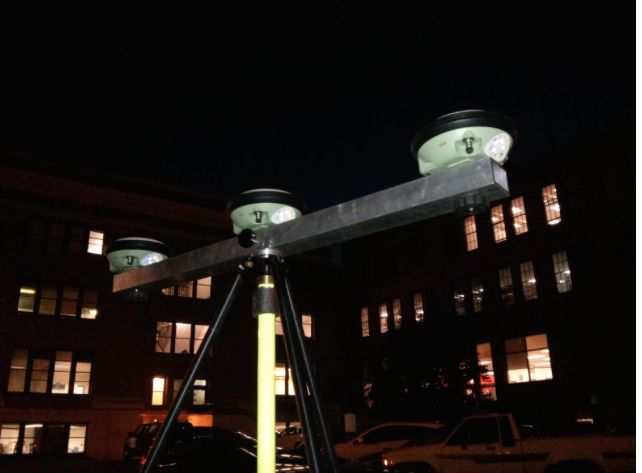
\includegraphics[width=500]{trident_title_pic}\par
\headingfont\bfseries\Large\@author\par
\bigskip\medskip
{\color{color2}\normalfont\normalsize\textbf{Project Summary:}\\
\getsummary}
\end{center}
\clearpage
}
\makeatother
%%%

%%% fancy boxes
\usepackage{tcolorbox}
\usepackage{wrapfig}
\def\fullboxbegin{
\bigskip
\begin{tcolorbox}[colback=color1,colframe=color1,coltext=white,arc=0mm,boxrule=0pt]
}
\def\fullboxend{\end{tcolorbox}\medskip}
%
\def\leftboxbegin{
\begin{wrapfigure}{l}{0.5\textwidth}
\begin{tcolorbox}[colback=color1,colframe=color1,coltext=white,arc=0mm,boxrule=0pt]
}
\def\leftboxend{
\end{tcolorbox}
\end{wrapfigure}
}
%
\def\rightboxbegin{
\begin{wrapfigure}{r}{0.5\textwidth}
\begin{tcolorbox}[colback=color1,colframe=color1,coltext=white,arc=0mm,boxrule=0pt]
}
\def\rightboxend{
\end{tcolorbox}
\end{wrapfigure}
}
%
\newcounter{frames}
\def\frameboxbegin#1{
\bigskip
\refstepcounter{frames}
\begin{tcolorbox}[colback=white,colframe=color1,arc=0mm,title={\MakeUppercase{\textbf{Frame \arabic{frames}}: #1}}]
}
\def\frameboxend{
\end{tcolorbox}
}
%%%

\usepackage{lipsum}

%%%%%%%%%%%%%%%
% Title Page
\title{Trident GPS System }
\author{Daniel Lin, Albert Le, and Nathan Christopher\\ Department of Civil Engineering \\ Oregon State University.}
\summary{
We developed an algorithm to help surveyors identify and remove multipathing GPS data points. We were able to test our algorithm with surveyors under real conditions and help surveyors become more productive during data surveying. 
}
%%%%%%%%%%%%%%%

\begin{document}
\maketitle

\tableofcontents
\clearpage

\section{Introduction}
\subsection{Client Information}
We worked with Dr. Dan Gillns from the Geomatics research group in the Department of Civil Engineering at Oregon State University. The project was requested by one of Dr.Gillns's grad student, Mike Eddy. This project is important because surveyors need a tool to be able to accurately determine their survey location. The accuracy of the surveyor's location data will determine the quality of the survey result. 

Our team consists of Daniel Lin, Nathan Christopher, and Albert Le, all Computer Science majors. Albert and Nathan were the primary develoers of the core algorithm of this project and Daniel is responsible for assisting the surveyors in field testing the algorithm and collecting and analyzing the data. Our client's role in our project is to help us analyze the result produced by our algorithm, assist us in composing the multipathing algorithm, and equipment management. 
\subsection{Project Background}
For well over a decade, surveyors have relied on survey-grade GPS to obtain accurate positioning data on earth. Recent technological advances have allowed surveyors to use advanced GPS positioning techniques called Real Time Kinematics (RTK) to obtain accurate GPS data in real time. One of the disadvantages of RTK include unreliability when under or near obstructions such as trees or buildings. The reason is that those obstructions act as a deflection shield; they deflect satellite signals away from a surveyor’s position, or cause the signal to bounce back and forth before reaching the GPS unit. This causes the position data of the surveyor to appear much further from the satellite than it is in reality, creating inaccuracies in position readings. This phenomena is called multipathing, and is a ubiquitous problem for surveyors.

The proposed solution of the client to solve the multipathing problem of RTK is to construct a fixed length physical rail. On the rail, there are attachment points for up to three GPS units, each positioned at a fixed distance away from each other. The idea is to place up to three Leica GPS receivers on the rail. One of the receivers will be placed in the middle of the rail, with the two others on either side of it to verify the middle receiver’s transmission data. If all three receivers’ transmitted data align with one another, then we can guarantee accurate GPS data are being broadcasted from the middle receiver.

In addition to eliminating the possibility of multipathing, there could be an added benefit of increased accuracy. Current accuracy levels range from decimeters to meters. As a byproduct of this project, the accuracy levels could drop down to centimeters.
\subsection{Problem Statement}

Our task is to design a program that is able to receive GPS data streams simultaneously from three Leica Viva GS14 receivers via usb to a portable device, or if possible via bluetooth to a mobile device. The program then parses the GPS receiver data in NMEA format and checks whether the GPS data is aligned or not. If it is not aligned or the data is not within the tolerance defined by the surveyor, then there is multipathing with the data and the program will not inform the surveyor to collect and save the GPS coordinates. If the receiver data is aligned, then the program informs the surveyor to save the coordinate data.  
 
The software should permit users to specify differing tolerances for vertical and horizontal shift among the GPS receivers, and allow users to specify the expected distance between GPS units, with the default being 0.5 meters. The software would display to the user, at a minimum, alignment status, longitude (in degrees, minutes and seconds), latitude (in degrees, minutes and seconds), and altitude (in meters).   
 
We are also tasked in constructing a user-friendly GUI for the program that allow surveyors to specify the distance between the GPS units mounted on the Trident and the tolerance levels of the data to determine if the data transmitted from the GPS receivers are aligned or not. 
 
The final requirement is that the program must be able to receive data in real time. Specifically, the program must be able to parse data transmitted by the receivers in real time and displayed to the user. 
 
If time and technology permits, the client would also like to have a webcam mounted upwards on the Trident system, taking a picture of the survey location and analyzing the percentage obstruction, the location of the obstruction (geographically), and the maximum angle the site permits.  
\clearpage
\subsection{Project Requirements}
\subsubsection{Team Requirements}
\begin{itemize}
\item User settable GPS spacing (in meters) 
\item User settable horizontal tolerance (in meters) 
\item User settable vertical tolerance (in meters) 
\item Software will allow for GPS connection in two different ways, Bluetooth and USB 
\item User Interface to interact with software 
\item Detailed manual on how to operate software 
\item Software outputs real-time data and presence of multipathing 
\end{itemize}
\subsubsection{Team Requirements}
\begin{itemize}
\item User predefined GPS receiver selection and orientation 
\item Software will scan all COM ports to connect GPS receivers on demand 
\item Software handles GPS timeouts and signal loss 
\item Software will receive NMEA GGA message 
\item Software will check for fixed position of GPS receiver, GGA GPS Quality Indicator value of 4 
\item Software converts longitude and latitude from degrees and minutes to degrees and decimal degrees 
\item Software will convert GPS latitude and longitude values into Cartesian coordinates via Oregon State Plane Coordinate System calculation 
\item Determine multipathing via single dot product calculation within calculated tolerance  
\item Determine multipathing via average dot product calculation within calculated tolerance 
\item Determine multipathing via linear tolerance check within given tolerance 
\item Determine multipathing via outlier check, 70 percent of minimum threshold 
\item Determine multipathing via linear altitude tolerance check within given tolerance 
\item User interface allows user to set tolerance levels, GPS connection settings and GPS receiver information 
\item User interface outputs real-time tolerance graph and real-time data 
\item User interface has API for alternate Cartesian coordinate conversion algorithm 
\item User interface allows for initialization of data logging 
\item User interface displays optional information from collected data, number of connected satellites, time data was collected, Geoidal Separation, etc. 
\end{itemize}
\subsubsection{Gantt Chart}

\section{New Requirements}
\begin{center}
\begin{tabu} to 0.8\textwidth { | X[l] | X[c] | X[r] | }
 \hline
 New Requirements & What Happened & Comments \\
 \hline
 This is a new req & item 22  & item 23  \\
\hline
\end{tabu}
\end{center}
\clearpage
\section{Blog posts}

\begin{figure}[H]
\centering
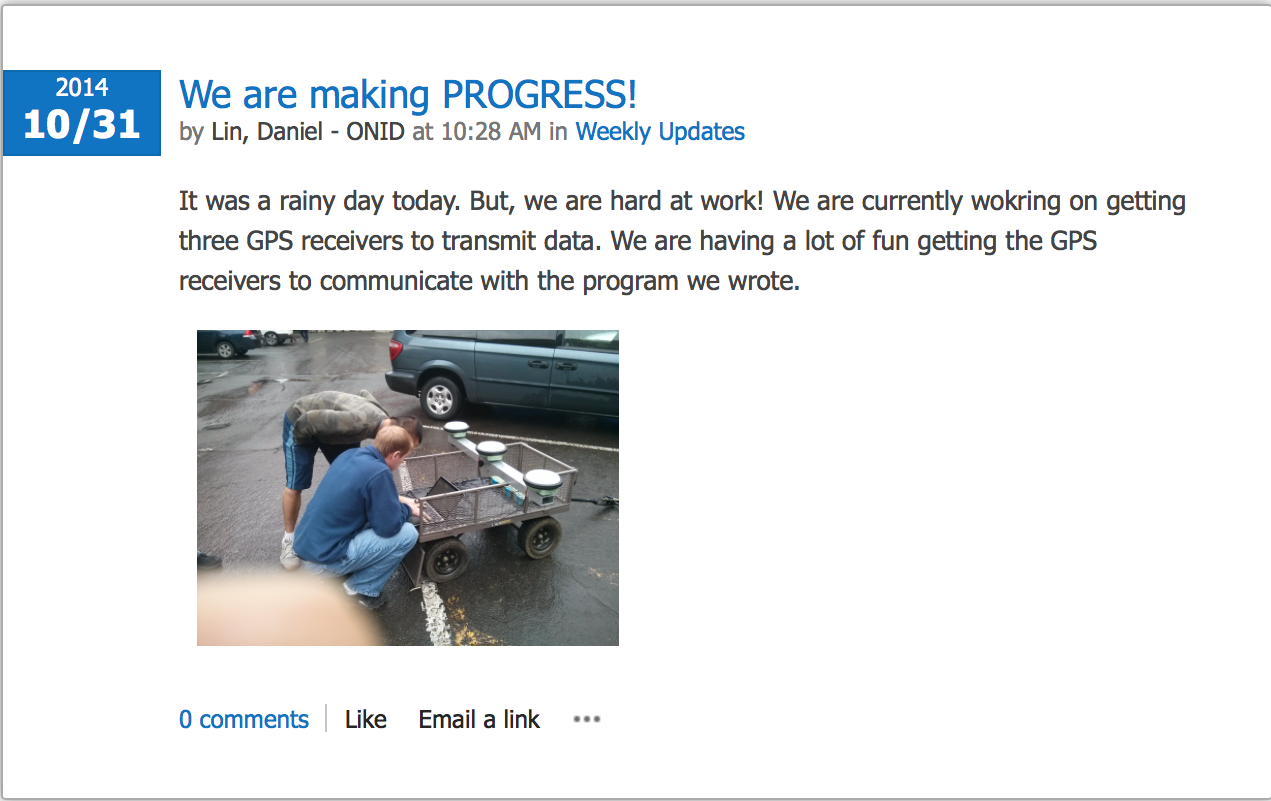
\includegraphics[scale=0.5]{blog_posts/2014_10_31.png}
\end{figure}

\begin{figure}[H]
\centering
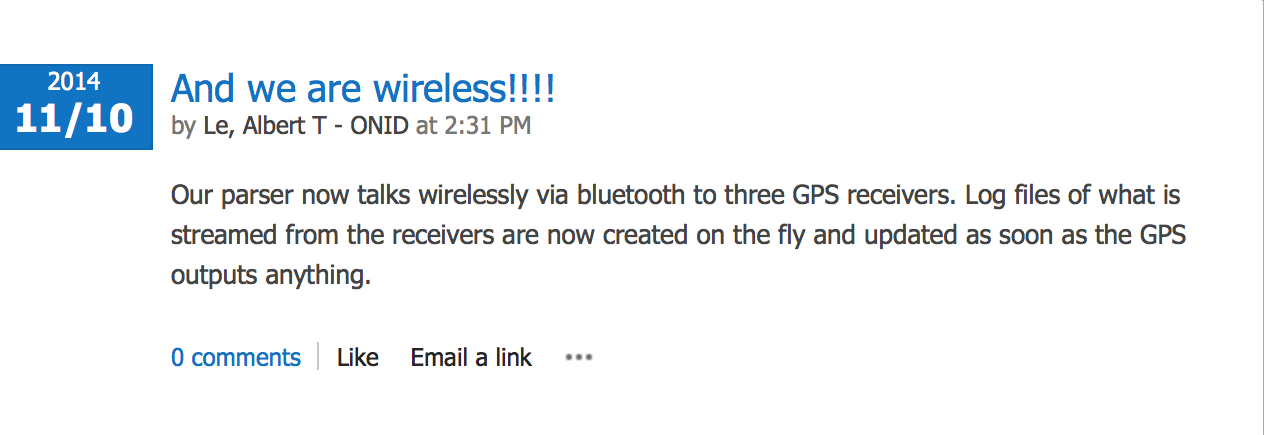
\includegraphics[scale=0.5]{blog_posts/2014-11_10.png}
\end{figure}

\begin{figure}[H]
\centering
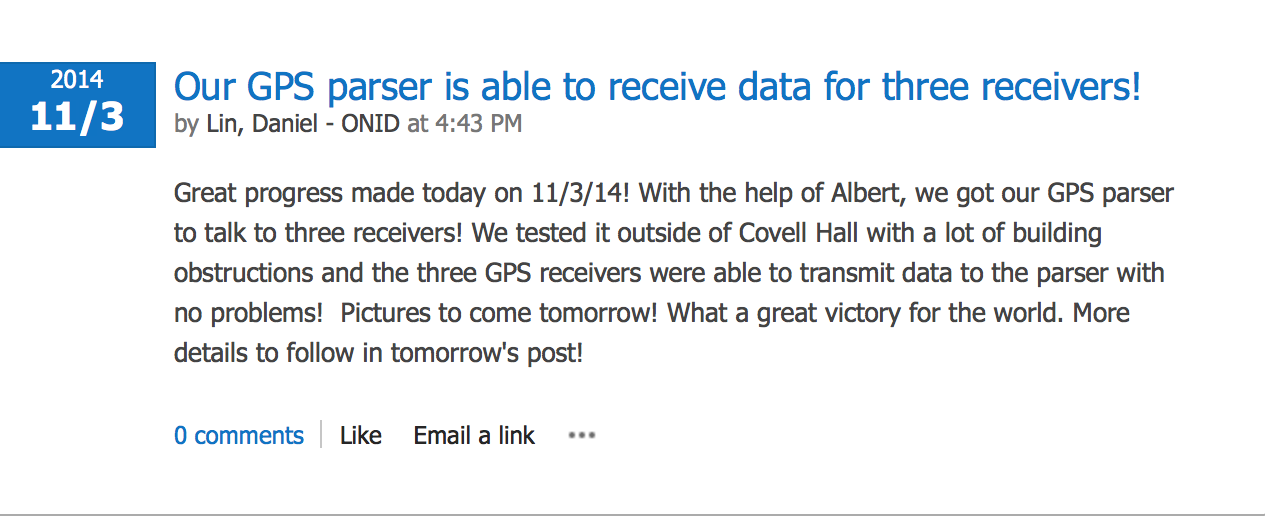
\includegraphics[scale=0.5]{blog_posts/2014_11_3.png}
\label{fig:my_label}
\end{figure}

\begin{figure}[H]
\centering
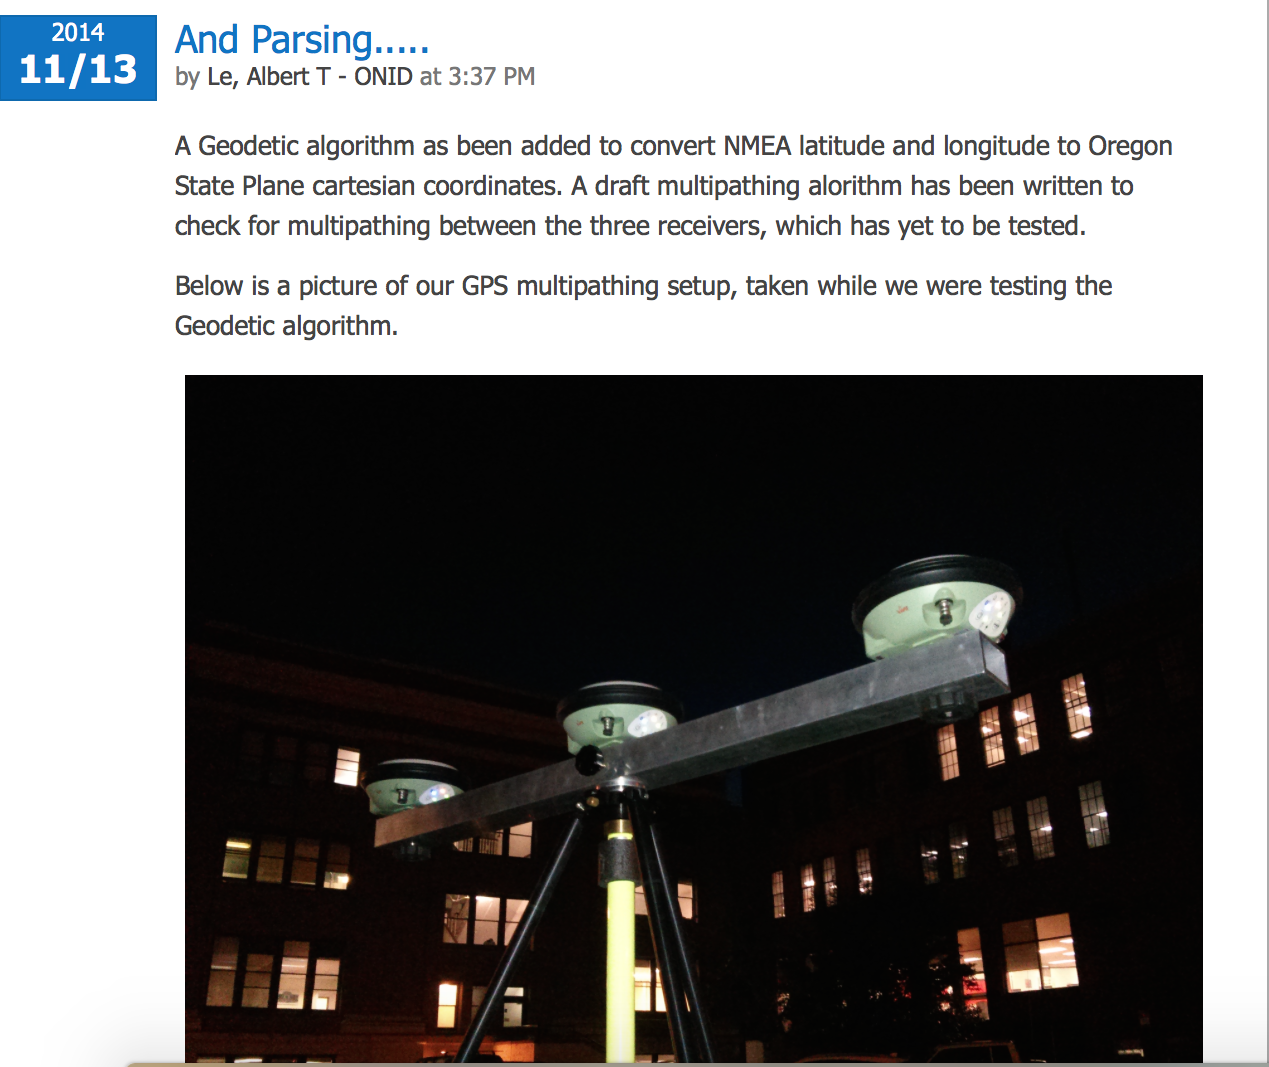
\includegraphics[scale=0.5]{blog_posts/2014_11_13.png}
\label{fig:my_label}
\end{figure}

\begin{figure}[H]
\centering
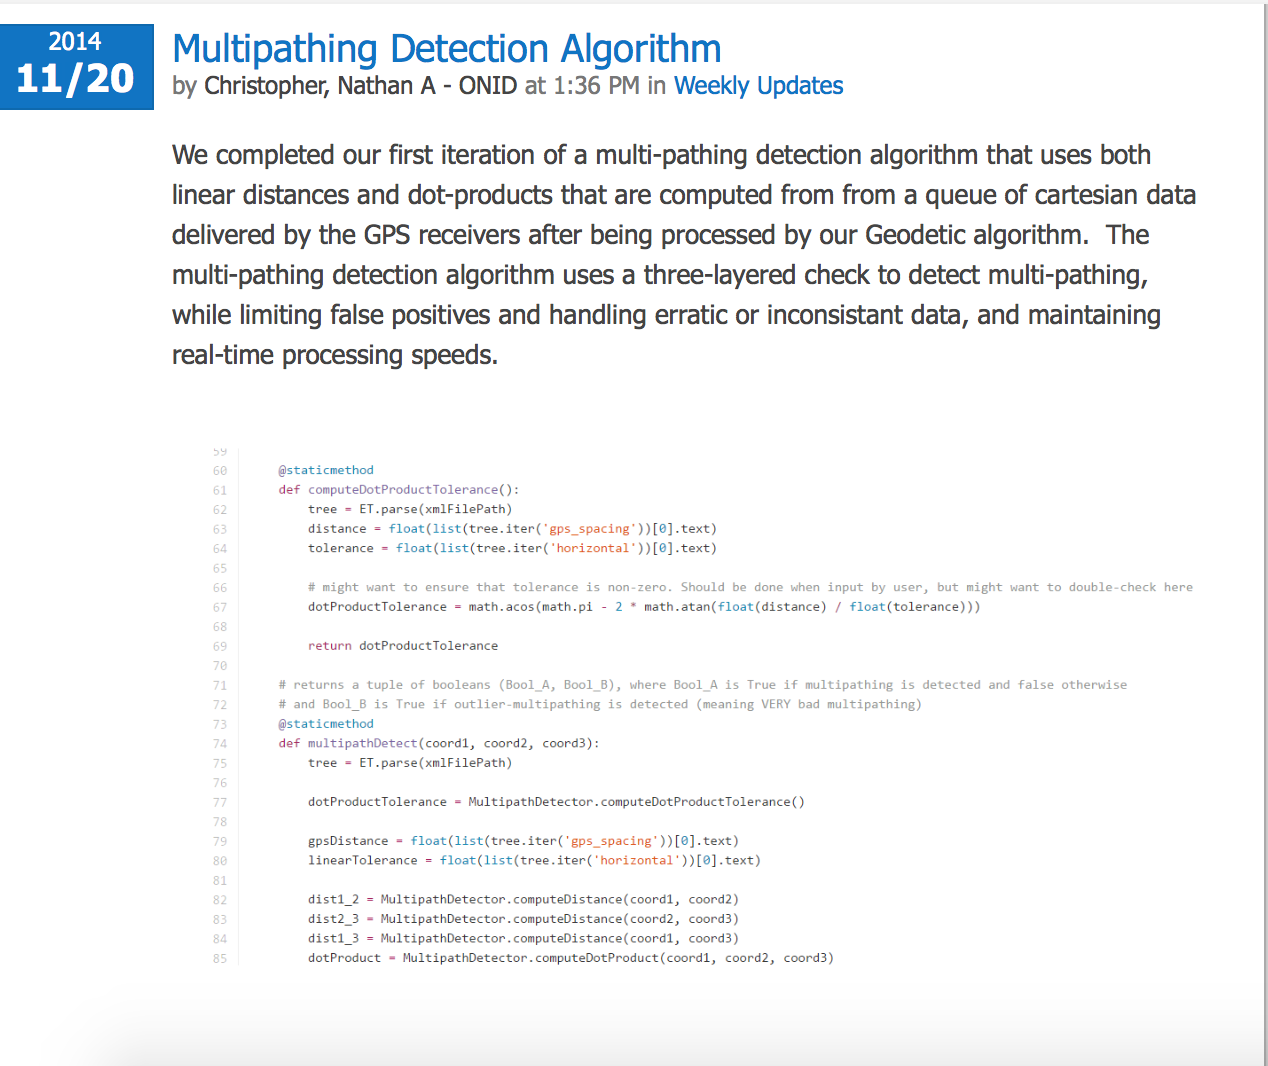
\includegraphics[scale=0.5]{blog_posts/2014_11_20.png}
\end{figure}

\begin{figure}[H]
\centering
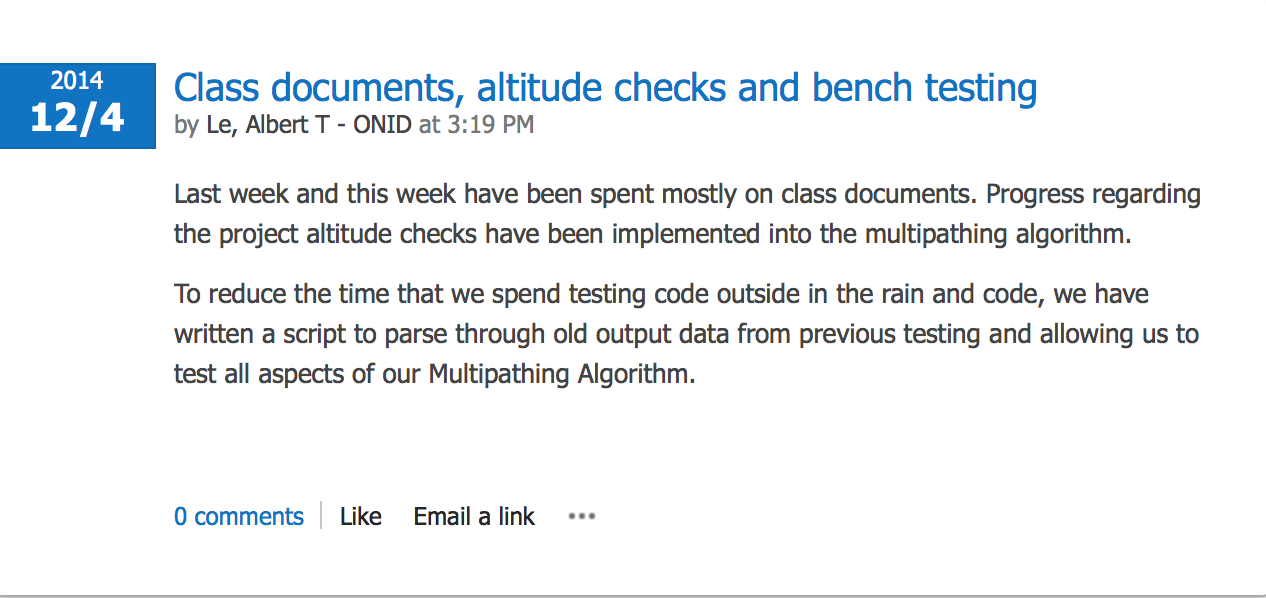
\includegraphics[scale=0.5]{blog_posts/2014_12_4.png}
\label{fig:my_label}
\end{figure}

\begin{figure}[H]
\centering

\includegraphics[scale=0.5]{blog_posts/2014_12_11.png}
\end{figure}

\begin{figure}[H]
\centering

\includegraphics[scale=0.5]{blog_posts/2015_1_9.png}
\end{figure}

\begin{figure}[H]
\centering

\includegraphics[scale=0.5]{blog_posts/2015_1_16.png}
\label{fig:my_label}
\end{figure}

\begin{figure}[H]
\centering
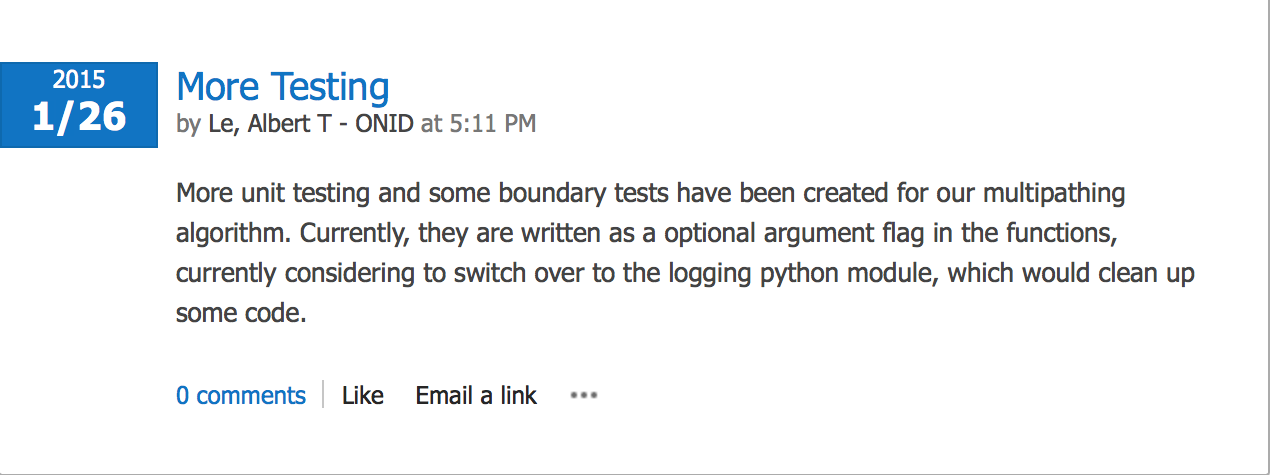
\includegraphics[scale=0.5]{blog_posts/2015_1_26.png}
\label{fig:my_label}
\end{figure}

\begin{figure}[H]
\centering
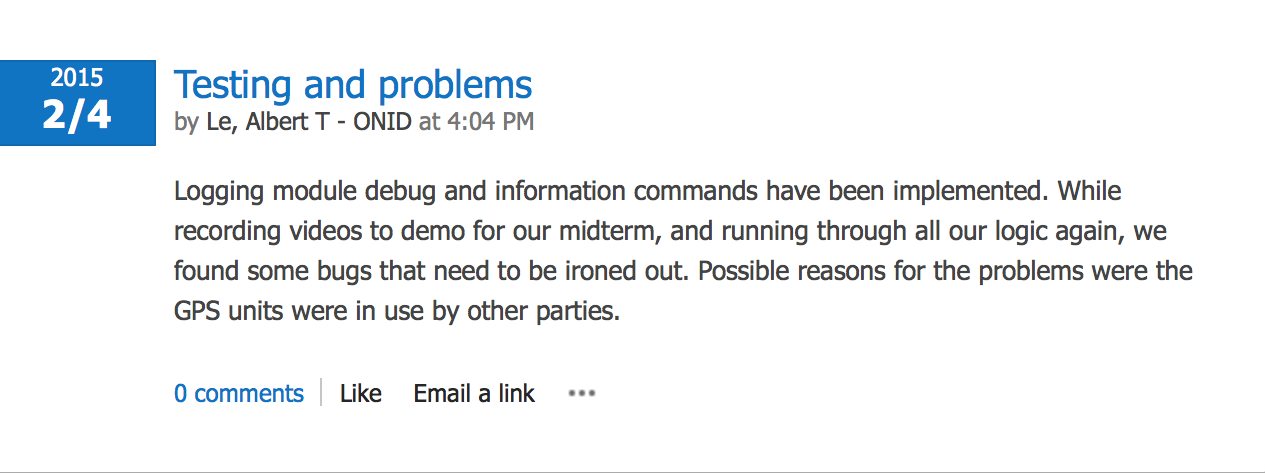
\includegraphics[scale=0.5]{blog_posts/2015_2_4.png}
\label{fig:my_label}
\end{figure}

\begin{figure}[H]
\centering

\includegraphics[scale=0.5]{blog_posts/2015_2_10.png}
\label{fig:my_label}
\end{figure}

\begin{figure}[H]
\centering
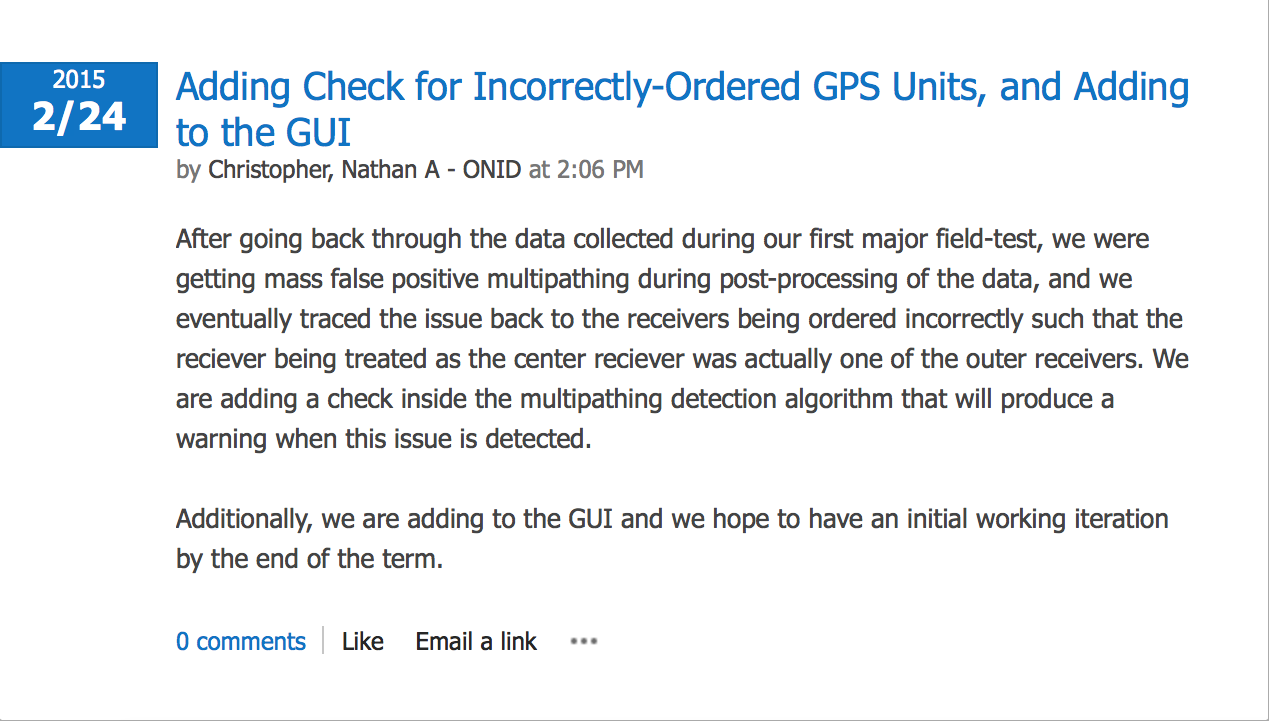
\includegraphics[scale=0.5]{blog_posts/2015_2_14.png}
\label{fig:my_label}
\end{figure}

\begin{figure}[H]
\centering
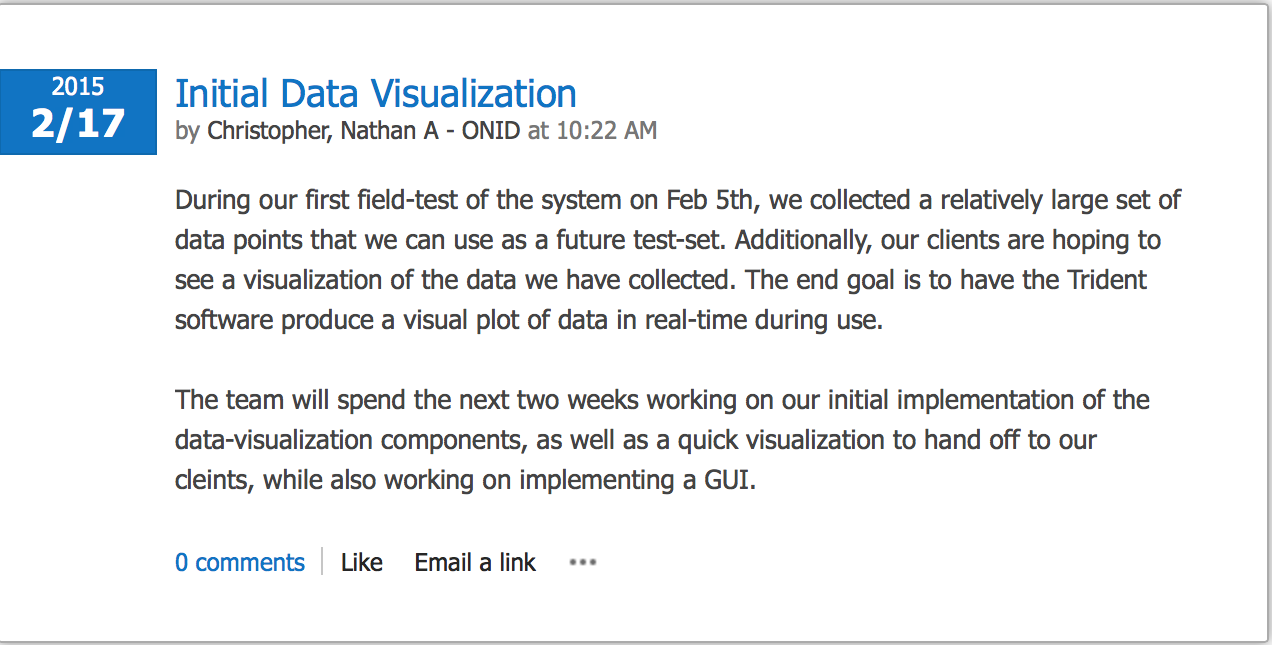
\includegraphics[scale=0.5]{blog_posts/2015_2_17.png}
\label{fig:my_label}
\end{figure}

\begin{figure}[H]
\centering
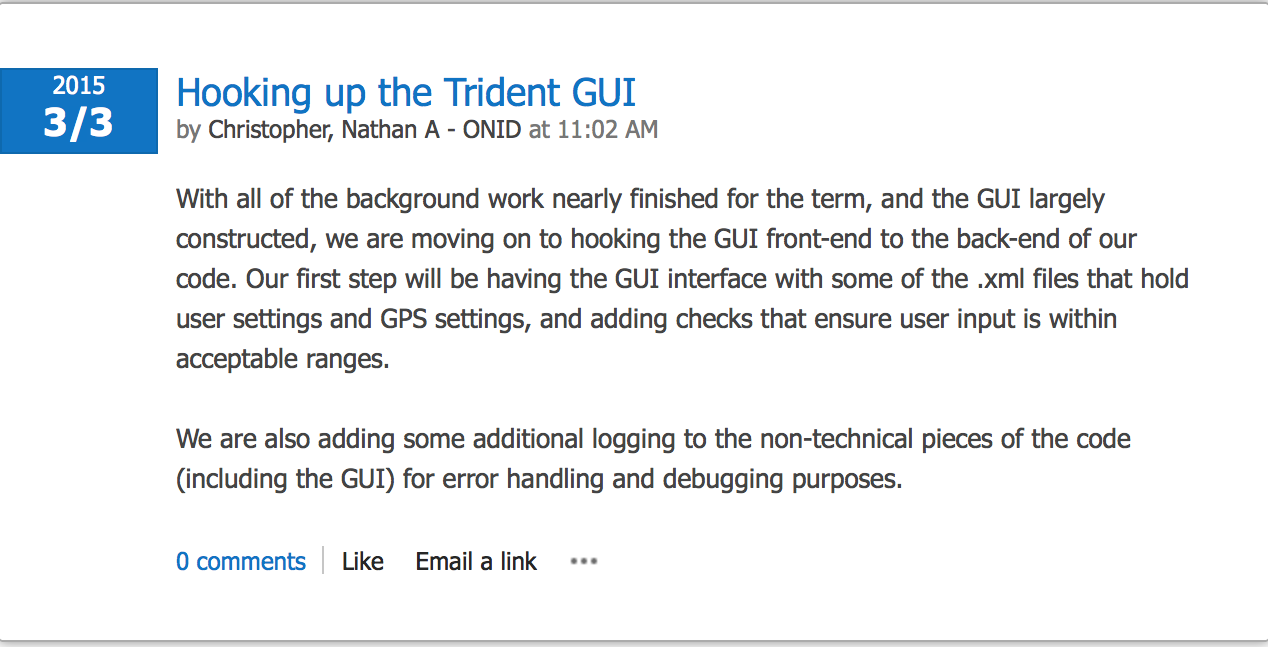
\includegraphics[scale=0.5]{blog_posts/2015_3_3.png}
\label{fig:my_label}
\end{figure}

\begin{figure}[H]
\centering
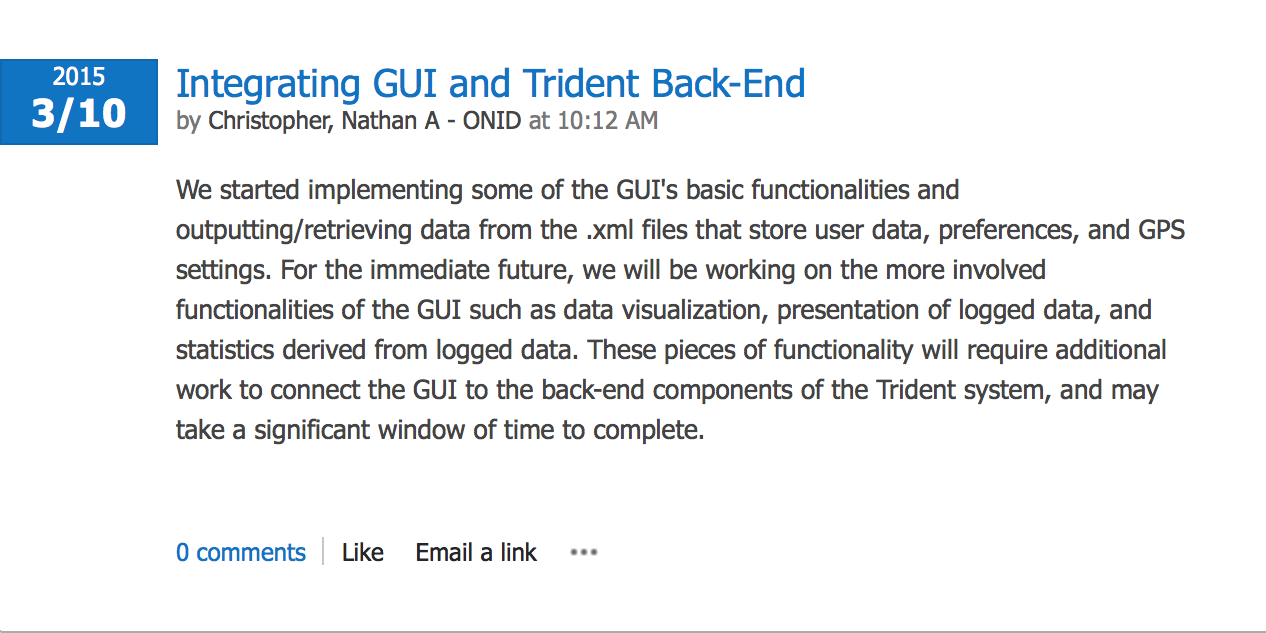
\includegraphics[scale=0.5]{blog_posts/2015_3_10.png}
\label{fig:my_label}
\end{figure}

\begin{figure}[H]
\centering
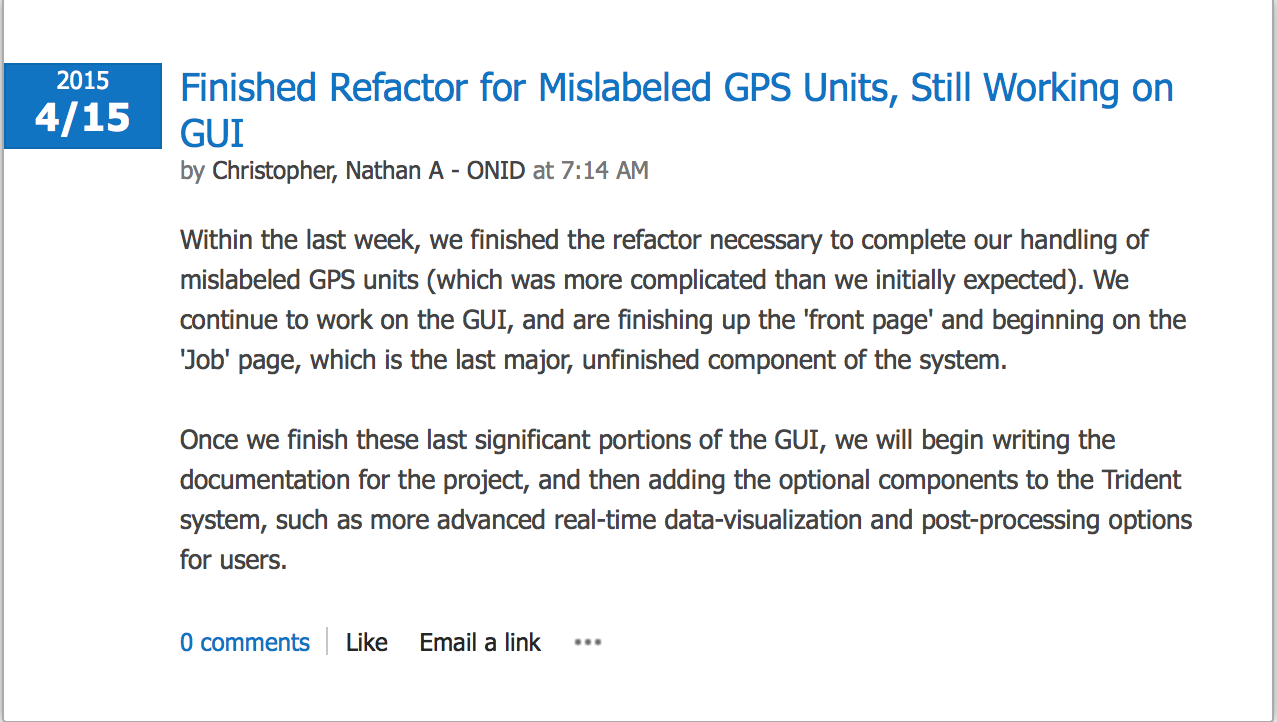
\includegraphics[scale=0.5]{blog_posts/2015_4_15.png}
\label{fig:my_label}
\end{figure}

\begin{figure}[H]
\centering
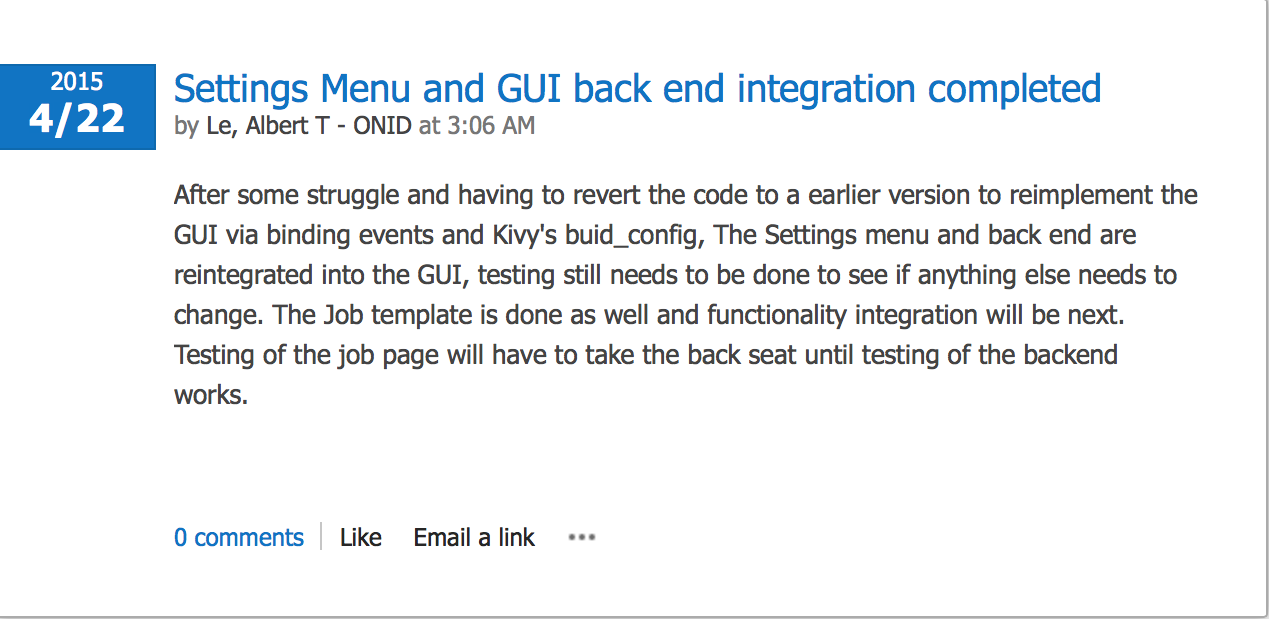
\includegraphics[scale=0.5]{blog_posts/2015_4_22.png}
\label{fig:my_label}
\end{figure}

\begin{figure}[H]
\centering
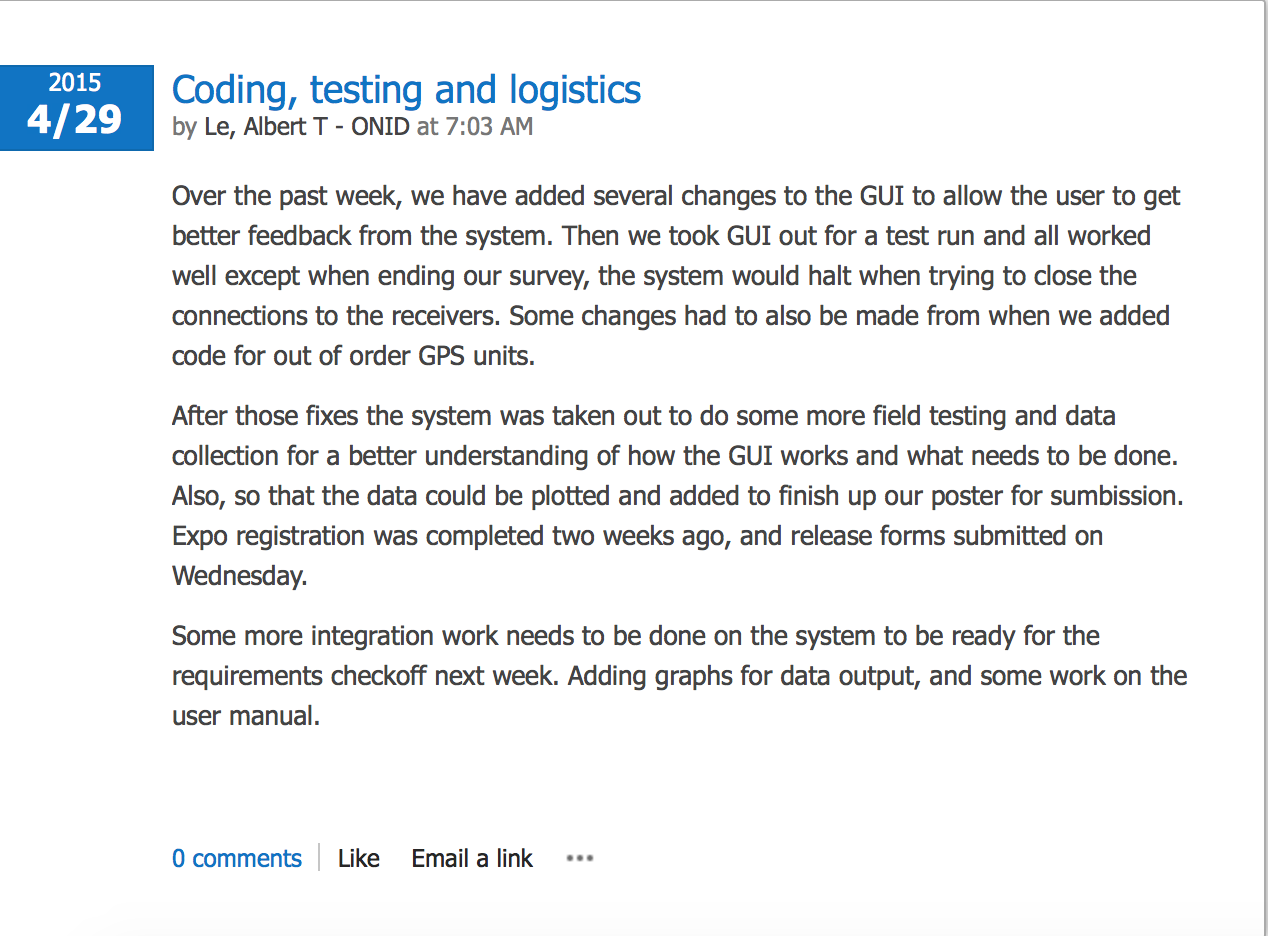
\includegraphics[scale=0.5]{blog_posts/2015_4_29.png}
\label{fig:my_label}
\end{figure}

\begin{figure}[H]
\centering
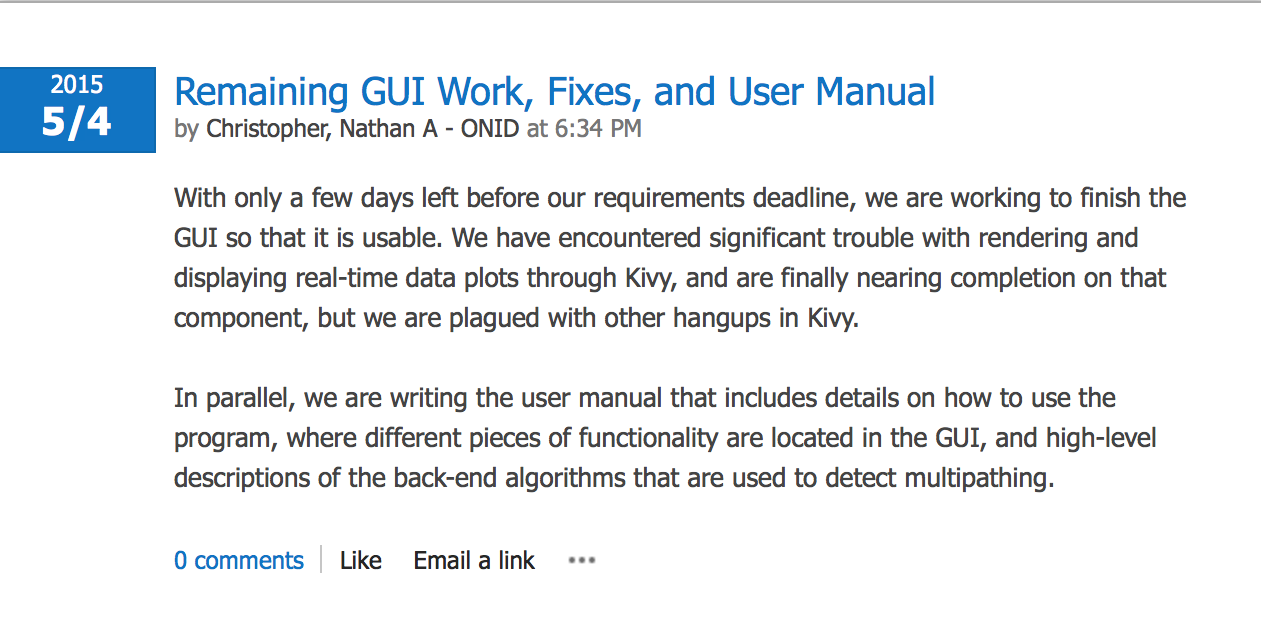
\includegraphics[scale=0.5]{blog_posts/2015_5_4.png}
\label{fig:my_label}
\end{figure}

\begin{figure}[H]
\centering
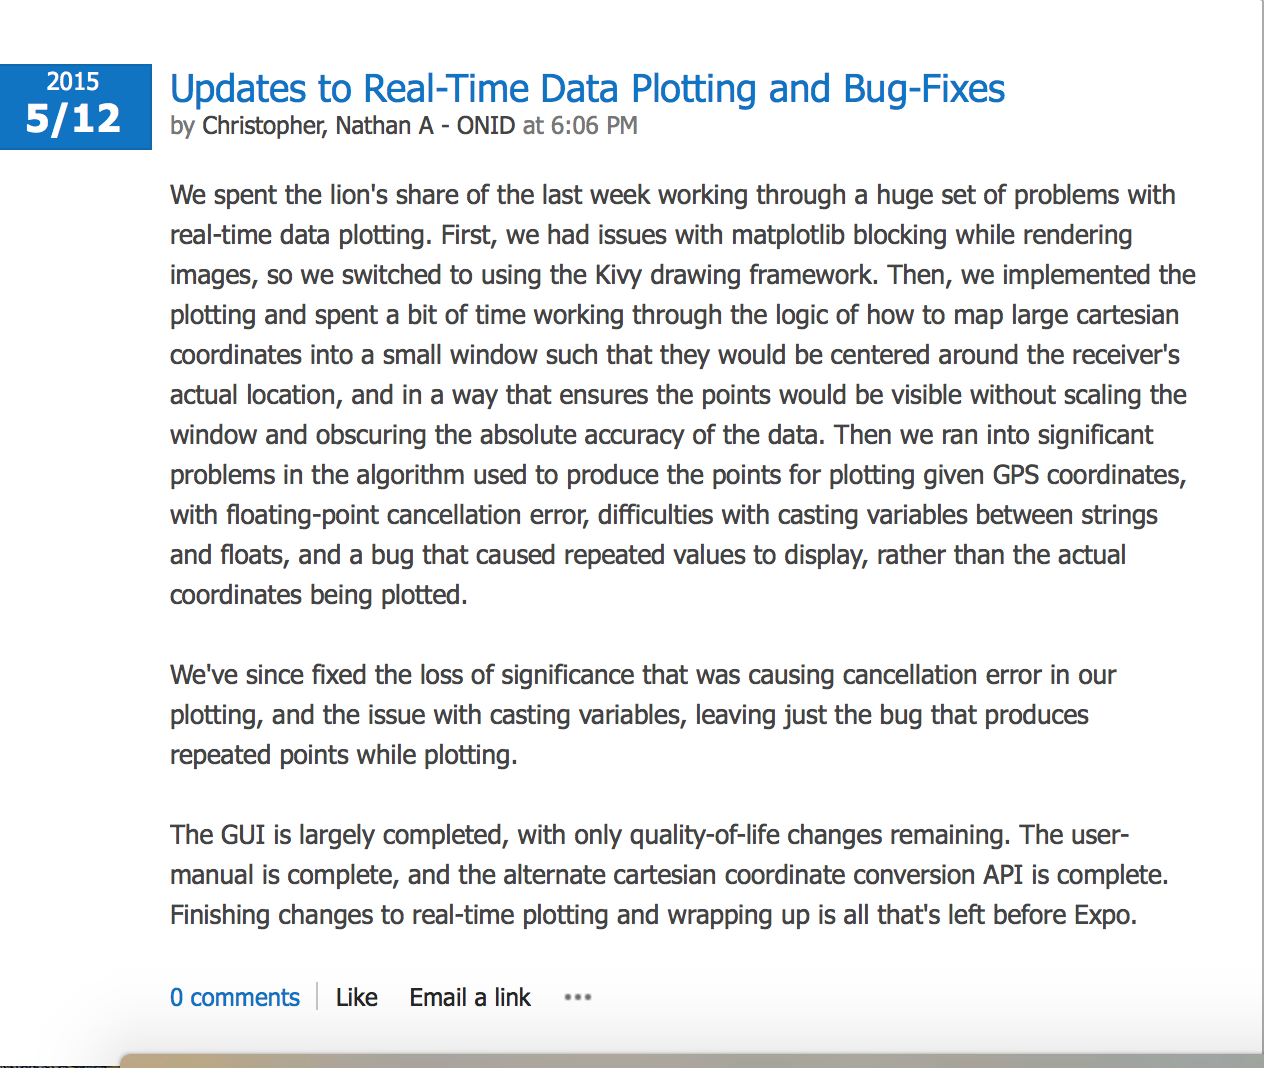
\includegraphics[scale=0.5]{blog_posts/2015_5_12.png}
\label{fig:my_label}
\end{figure}

\begin{figure}[H]
\centering

\includegraphics[scale=0.5]{blog_posts/2015_5_20.png}
\label{fig:my_label}
\end{figure}

\begin{figure}[H]
\centering

\includegraphics[scale=0.5]{blog_posts/2015_5_27.png}
\label{fig:my_label}
\end{figure}

\section{Project Description}
\subsection{How does our project work?}
The first step in operating on a data epoch obtained from the receivers is to convert latitude and longitude into cartesian coordinates. This is necessary to enable the Trident’s multipathing detection algorithms to operate on the data. By default the Trident system converts latitude and longitude to the Oregon State Plane Coordinate System; however, the Trident system is extensible and has an API for alternate coordinate systems that would allow the Trident system to convert latitude and longitude to any other set of cartesian coordinates.

The Trident system uses a series of algorithms to check each data epoch for multipathing, including a linear distance check, an altitude comparison, and an assessment of the dot product of the angle formed by the three receivers.

The algorithm first uses a  linear distance check of the cartesian coordinates of the three receivers to filter multipathing data. Each receiver’s x- and y-coordinates are used to compute the horizontal linear distance between each combination of two receivers by using the standard cartesian distance formula. The computed linear distance is compared to the fixed physical distance between each receiver. If the computed horizontal distance is further from the known physical distance than the permitted linear tolerance, then the data epoch is labeled as multipathing.

Next, a linear distance comparison of the altitude of the three receivers checks for anomalous vertical positioning data. The difference in altitude between each combination of two receivers is computed. If the difference in computed altitude is greater than the specified altitude-tolerance, then the data epoch is labeled as multipathing. It is noteworthy that this algorithm requires that the Trident system stands perfectly vertically such that the receivers are at the same physical altitude.

Finally, a dot product check of the angle formed by the three receivers is used. First, a dot product tolerance is derived mathematically from the horizontal linear tolerance. Then, the dot product of the angle formed by imaginary lines drawn through the left and center receivers and the right and center receivers is computed. The resulting dot product is compared to the derived dot product tolerance, and epochs are labeled as multipathing if the computed dot product is outside of the allowed tolerance.

The relationship between the linear horizontal distance and the dot product checks is of significant importance. Because the dot product tolerance is derived from the linear horizontal tolerance, the combination of the linear horizontal distance test and the dot product test ensures that an epoch which passes both tests is mathematically guaranteed to contain cartesian coordinates such that each receiver’s perceived location must be within the linear horizontal tolerance of its known location relative to the other receivers. In short, the dot product test combined with the linear distance test produces a composite test that compares each receiver’s perceived location with its actual location relative to the other receivers.

Each data epoch is checked for multipathing using the multipathing detection algorithms twice: the first time using the exact cartesian coordinates produced by that epoch, and the second time using the averaged cartesian coordinates produced by that epoch and the nine epochs immediately prior to the current epoch. The detection of multipathing via both these methods is recorded alongside the GPS data, and is used in later checks that ultimately determine what data the Trident system labels as inaccurate.

After the multipathing algorithms operate on each data epoch, and each queue of ten data epochs, further checks are done by assessing the data epochs in the queue of the ten most recent data epochs. If three or more of the epochs within the queue show multipathing individually, then the current point will be labeled as multipathing as an additional filter to help constrain the inclusion of potentially bad data in locations with heavy multipathing. Additionally, if any perceived location in the queue was three or more times the tolerance away from its physical location, the most recent data epoch will be labeled as multipathing as yet another additional filter to help ensure that data of poor quality does not impact the final result. These combined criteria have proved to nearly guarantee a high quality of data, and high accuracy, and produce clean results even in areas of heavy multipathing. Note that the labeling of epochs as multipathing due to these checks is not carried over to the next check. That is, each time a new queue is evaluated, points that were labeled as multipathing previously due to the contents of their associated queue will only be evaluated by their individual multipathing status, not their queue-based multipathing status, so heavy multipathing will not necessarily cascade in a way that labels all future data as multipathing.

To help users assess the quality of the data, and inform them of the severity and frequency of multipathing at a location, the number of epochs labeled as multipathing at a given point and the number of total epochs collected at that point are tracked by the Trident, and their ratio is displayed while surveying a point. Points where more than than approximately 50 percent of the epochs are detected as multipathing should generally be considered unreliable. The filtered, cleaned data collected from these points by the Trident will still be reliable, but the percentage of multipathing epochs gives a good measure of the stability of the data gathered at that location.
\section{Typical Workflow of the project}
A typical workflow for a survey might look like the following:
\begin{itemize}
\item Turn on GPS units, and configure them appropriately, making sure to double-check the antenna height setting for each receiver, which can cause problems for the Trident’s multipathing algorithms if they are not all set to the same height.
\item Set up the Trident at the point to be surveyed. Make certain that the Trident is perfectly level.
\item Start the Trident software system.
\item Open the settings menu, and select the appropriate receivers. Set the tolerances to your preference, and set the antenna height and phase center offset settings appropriately.
\item Set the survey name
\item Begin the survey
\item Add a point, and enter the name for the current location being surveyed. Specify the optional point code if desired.
\item When the receiver status indicators indicate that the GPS units are connected to the Trident system, begin collecting data by pressing ‘Measure Point’
Allow the system to collect as many epochs as desired. The current number of epochs collected is displayed near the bottom right-hand corner of the screen, alongside the number of epochs detected as multipathing, and the percentage of multipathing epochs among all epochs collected.
\item Click ‘Stop’
\item Navigate to the output folder, and the subdirectory with the same name as the current survey. Locate the CSV file with the name of the current point. Open the file and inspect the results.
\item Move to a new location, and repeat the steps to set up the Trident, add a new point, and begin surveying. Repeat as necessary. When data for all points in the survey has been collected, click ‘End Survey’.
\item Close the Trident software system. Make any necessary backups of the CSV output files produced for this survey. Have a beer and high-five your buddy.
\end{itemize}

\section{Project Documentation}
\subsection{Front End} 
\begin{figure}[H]
\centering
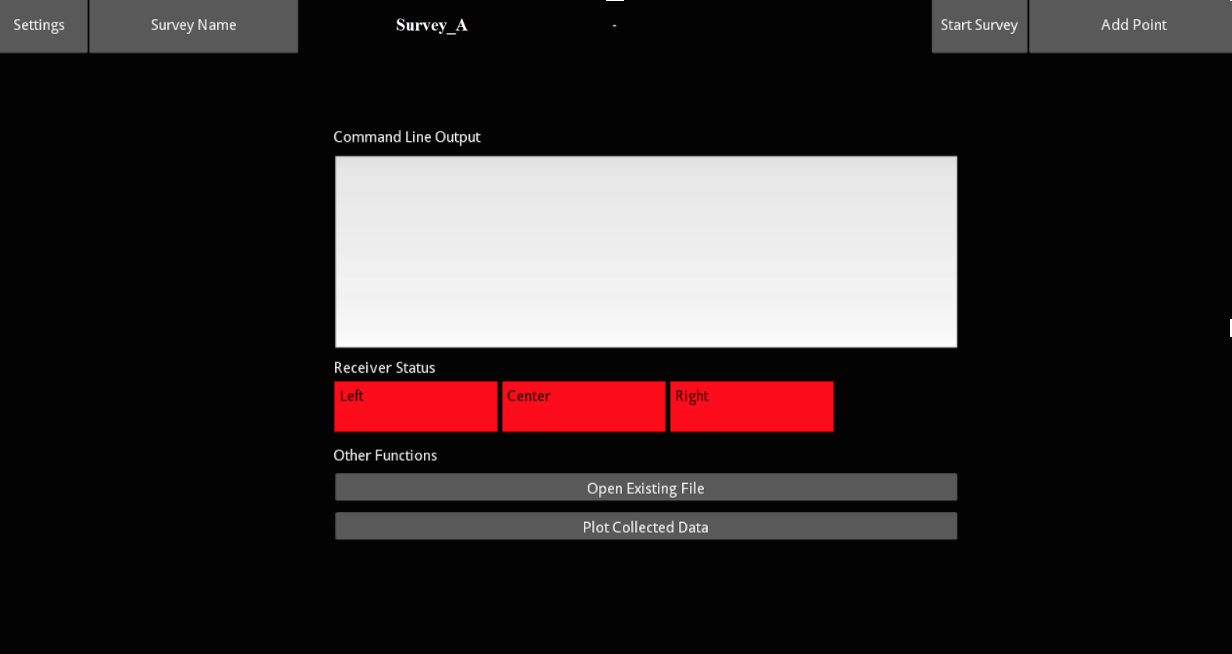
\includegraphics[scale=0.5]{blog_posts/GUI_1.png}
\caption{Front end of the GUI}
\label{fig:my_label}
\end{figure}
Below are the components of the Front end GUI: \\ \\
\textbf{Receiver Status Indicators:} \\ 
These three colored dots near the top right-hand corner of the screen indicate the status of the receivers specified in the Trident settings menu. The left bubble corresponds to the left receiver, the center bubble to the center receiver and so on, as defined in the Trident settings menu.Receivers that are connected will display as yellow, receivers that are connected and are receiving coordinate-quality 4 data will display as green, and receivers that are not connected will display as red. If no receivers are specified in the Trident settings menu, then the status indicators default to red. Clicking on one of the receiver indicators will open a display that shows information pertaining to that receiver, including the number of connected satellites, current coordinate quality, current perceived altitude, and current perceived latitude and longitude of the receiver. \\ \\
\textbf{Survey Name:} \\ 
Pressing this button prompts you to set the current survey name - use whatever name helps to identify this survey and distinguish it from others. Recall that each survey can contain multiple locations, or ‘points’ from which data can be collected. The current survey name is displayed to the immediate right of the ‘Survey Name’ button (see Figure 1, note the current survey name ‘Survey A’). NOTE: Once a survey is started, the settings in the Trident settings menu cannot be changed for that survey, so make sure that your settings are set correctly before beginning! \\ \\
\textbf{Start Survey:} \\ 
This button begins a survey. Points can now be added to this survey, and the current point name will be displayed to the immediate left of the ‘Start Survey’ button.NOTE: The Trident settings menu is locked once a survey is begun, so make sure that the settings are set appropriately before beginning a survey. \\ \\
\textbf{Add Point:} \\ 
Pressing this button prompts you to set the current point name and point code - use whatever name and code help to identify this point uniquely, making sure that it is easily distinguishable from other points within this survey.While data is not being collected for a point you can switch between all points within the current survey by swiping left or right.Once the point name has been set, the ‘Measure Point’ button will be unlocked. The ‘Measure Point’ button is located near the bottom right corner of that point’s page. \\ \\
\textbf{Measure Point:} \\ 
Pressing this button begins data collection for the current point within the current survey. Measurement will cease when the specified number of epochs have been collected, or when the ‘Stop Measurement’ button is pressed, whichever occurs first.NOTE: If any data has been collected for a point, pressing the ‘Measure Point’ button for that point a second time will overwrite all existing data from that point and begin a fresh data-set. All previous data will be lost.\\ \\
\textbf{Stop:} \\
This button appears after measurement has begun for a point. Clicking it will cease data collection for the current point, and cause the Trident to output the amortized results of all data collected for that point into a .csv file in the ‘outputs’ directory, within a subdirectory named with the survey’s name. All final output files will be stored in this fashion. \\ \\
\textbf{Data Plot:} \\ 
Pressing this button displays a graph of the cartesian coordinates of the center receiver’s perceived location in real time. The ten most recent data epochs from the center receiver are displayed. Blue dots indicate non-multipathing data, while red dots indicate that data has been declared as multipathing. NOTE: Altitude data is not displayed in this graph, and points whose altitude cause them to be declared as multipathing may appear to be clustered near non-multipathing data whose altitudes are within tolerance.
\subsection{Settings Menu}
\begin{figure}[H]
\centering
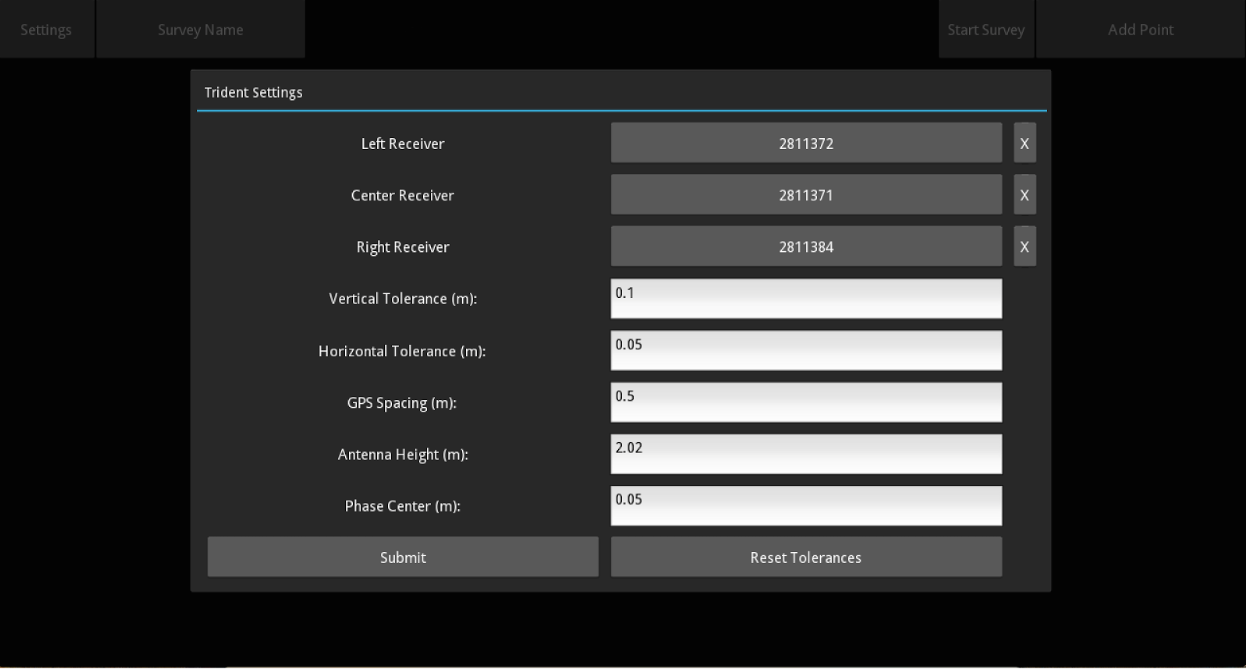
\includegraphics[scale=0.5]{blog_posts/GUI_2.png}
\caption{Settings menu for the GUI}
\label{fig:my_label}
\end{figure}
The top three entries in the Trident settings menu are responsible for selecting GPS receivers to which the Trident system will connect. Clicking on the drop-down menu for each the left, center, and right receivers reveals the list of known receivers to which the system can connect. No receiver can be selected for multiple positions. Clicking the ‘X’ to the right of each receiver’s drop-down menu will clear that drop-down menu, and a new receiver will need to be selected. Each receiver position must have a receiver selected in order to start a survey.\\ \\
NOTE: It is imperative that the center receiver is labeled as such. The ‘left’ and ‘right’ receivers are entirely interchangeable, and their ordering does not affect the Trident’s algorithms; however, if the wrong receiver is labeled as the center receiver, then the Trident’s algorithms will fail to process data properly. Such a mislabeling will be caught by the Trident’s algorithms, causing the system to cease data collection, and exit to the Trident main page after producing a message stating that the center receiver has been mislabeled. \\ \\
Below the receiver connection settings are the tolerance and distance settings. Here, you can set the various tolerances used by the Trident’s algorithms, as well as the fixed distance between the mounted receivers.
\subsubsection{Instructions to Run the Trident Software}

\section{Technology Review}
\textbf{What we are Trying to Accomplish} \\
Our goal is to find a way to gather NMEA data from 3 (or more) GPS receivers, parse that data, implement an algorithm to detect GPS multi-pathing from the parsed NMEA data, and design a GUI to display the presence of multi-pathing. \\ \\
\textbf{Possible Technologies} \\ 
In regards to connecting to the GPS receivers, we have several possible interfaces. One possible approach to the problem is using USB serial connections to connect the GPS receivers to a laptop. Another method is to use multiple bluetooth connections between the GPS receivers and a laptop or mobile device. The last method is creating a web server and communicating data from multiple GPS devices via the web.\\ \\
We decided to rule out the web method due to potential complications and a potential inability to send data from multiple GPS units. After speaking with one of our clients about his preferences, we decided to go with the bluetooth method because there was no significant monetary cost difference or implementation complexity difference between the bluetooth and USB methods. As a backup method, because of bluetooth connection problems, USB can be used as a backup option. Since both methods are handled the same, this entails no extra software work. \\ \\
Potential languages for the project include: Python, C/C++, PHP, and Perl. PHP and Perl would be ideal for the web server option; however, because of the web connectivity issues with the GPS units as well as our comfort level with these languages we decided to stay away from PHP and Perl. We eventually decided to go with Python because we liked the idea of more rapid development in comparison with C/C++, and no performance issues were anticipated. Additionally, Python has some really nice libraries and functionality that could ease the implementation of the project. Python also allows us to create interfaces to possible web and mobile frameworks. \\ \\
For GUI, we had a number of possible routes: A mobile app for Android, a website for a web server implementation, Python using the Kivy framework, or C with ASP.net. Ultimately, we decided to rule out a website due to the aforementioned reasons. Instead, we wanted to work solely in Python in keeping with our decision to use Python for the parser portion of the project.


\end{document}          
